\documentclass[../main.tex]{subfiles}
%\graphicspath{{\subfix{images/}}}
%\usepackage{xr}
%\externaldocument{../sections/introduction}
%\externaldocument{../sections/lwe}

\begin{document}

\label{section:lattice theory}
%\section{Lattice theory (light)}

\subsection{Lattice basics}

%Start with a review of some linear algebra concepts. 

%\textbf{Keywords: vector space, basis, span, linearly independent, matrix determinant, etc}


Lattices are useful mathematical tools for connecting different areas of mathematics, computer science and cryptography. They are widely used for cryptoanalysis and building secure cryptosystems. In this section, we will introduce the basics of lattices in the general setting $\R^n$. In addition, we introduce dual lattices and some computational lattice problems that are commonly used to achieve provable security of lattice-based hard problems and cryptosystems. At the end of this section, we will sketch \citet{ajtai1996generating}'s polynomial time worst-case-to-average-case reduction to reinforce our understanding of lattices as well as appreciate the great breakthrough in provable security of lattice-based cryptography, even against quantum computing in some cases. Although we introduce lattices in the most general setting, their results also hold for special lattices such as ideal lattices in the ring learning with error problem. 

Intuitively, a lattice is similar to a vector space except that it consists of discrete vectors only, that is, elements in lattice vectors have discrete values as opposed to real-valued vectors in a vector space. For example, Figure \ref{fig:lattice1} is a lattice in $\R^2$. More formally, we have the following definition. 

\begin{definition}
Let $\mathbf{v_1}, \dots, \mathbf{v_n} \in \R^m$ be a set of linearly independent vectors. The \textbf{lattice} \index{lattice} $L$
\reversemarginpar
\marginnote{\textit{Lattice}}
generated by $\mathbf{v_1}, \dots, \mathbf{v_n}$ is the set of integer linear combinations of $\mathbf{v_1}, \dots, \mathbf{v_n}$. That is, 
\begin{equation*}
    L = \{a_1 \mathbf{v_1} + \cdots + a_n \mathbf{v_n} \mid a_1, \dots, a_n \in \Z\}.
\end{equation*}
\end{definition}
Here, the difference with vector spaces is that the coefficients in the linear combination are integers. The integers $m$ and $n$ are the \textbf{dimension} and \textbf{rank} 
\reversemarginpar
\marginnote{\textit{Dimension, rank}}
of the lattice respectively. If $m=n$, then $L$ is a \textbf{full-rank} lattice. In most cases, we work with full-rank lattices. 

It follows from the definition that a lattice is closed under addition. Hence, we can say that an n-dimensional lattice is a discrete additive subgroup of $\mathbb{R}^n$. It is isomorphic to the additive group of $\mathbb{Z}^n$. That is, 
\begin{equation*}
    (L, +) \cong (\Z^n, +) \subsetneq (\R^n, +).
\end{equation*}

It is often convenient to work with lattices whose coordinates are integers. These are called \textbf{integer lattices} or \textbf{integral lattices}. 
For example, the set of even integers forms an integer lattice, but not the set of odd integers because it is not closed under addition. 

\begin{figure}[ht]
  \centering
  \includegraphics[page=2]{images/Lattice_crypto_tikz_folder.pdf}
  \caption{A lattice $L$ with a basis $B=\{b_1, b_2\}$ and its fundamental domain $F$.}
  \label{fig:lattice1}
\end{figure}


A \textbf{basis} \index{lattice! basis}
\reversemarginpar
\marginnote{\textit{Basis}}
of a lattice $L$ is a set of linearly independent vectors $B = \{b_1, \dots, b_n\}$ that spans the lattice, that is,
\begin{equation*}
    L(B)= \{z_1 b_1 + \dots + z_n b_n \mid z_i \in \mathbb{Z}\}.
\end{equation*}
For example, the vectors $\{b_1,b_2\}$ form a basis of the lattice in Figure \ref{fig:lattice1}.
\begin{figure}[ht]
  \centering
  \includegraphics[page=3]{images/Lattice_crypto_tikz_folder.pdf}
  \caption{The same lattice $L$ with a different basis $B'=\{b_1', b_2'\}$ and its fundamental domain $F'$, where $B'=AB$ for a unimodular change of basis matrix $A=\big(\begin{smallmatrix}
  1 & 1\\
  1 & 2
\end{smallmatrix}\big)$.}
  \label{fig:lattice2}
\end{figure}

In what follows, we will frequently appeal to properties of a class of matrices known as \emph{unimodular matrices}. Unimodular matrices can be used to translate between different lattice bases. They are also used, sometimes implicitly, when performing important lattice operations such as lattice basis reduction.
\begin{definition}
\reversemarginpar
\marginnote{\textit{Unimodular matrix}}
A matrix $A \in \Z^{n\times n}$ is \textbf{unimodular} if it has a multiplicative inverse in $\Z^{n\times n}$. That is, $A \in \Z^{n\times n}$ is unimodular if and only if $A^{-1} \in \Z^{n\times n}$. Equivalently, a matrix $A \in \Z^{n\times n}$ is unimodular if and only if $|\det(A)| = 1$.
\end{definition}

Similar to a vector space, a lattice does not need to have a unique basis. The following proposition establishes the fact that one basis can be transformed to another via multiplication by the matrix $A$ provided that $A$ is a unimodular matrix.
\begin{proposition}
If $B$ and $B^{\prime}$ be two basis matrices, then $L(B) = L(B^{\prime})$ if and only if $B^{\prime} = AB$ for some unimodular matrix $A$.
\end{proposition}
\begin{proof}
Suppose that $B^{\prime} = AB$ for some unimodular matrix $A$. Then, by definition both $A$ and $A^{-1}$ have integer entries.  Therefore we have $L(B^{\prime}) \subset L(A^{-1}B^{\prime}) = L(B)$ and $L(B) \subset L(AB) = L(B^{\prime})$.

Now suppose that $L(B) = L(B^{\prime})$. Then there exist integer square matrices $A, A^{\prime} \in \Z^{n \times n}$ such that $B^{\prime} = AB$ and $B = A^{\prime}B^{\prime}$. Therefore we have $B = A^{\prime}AB$ or equivalently $(I - A^{\prime}A)B = 0$. Because $B$ is nonsingular, we have $A^{\prime} = A^{-1}$ and $A$ is unimodular.
\end{proof}

For example, the vectors $\{b_1',b_2'\}$ in Figure \ref{fig:lattice2} form a different basis for the lattice in Figure \ref{fig:lattice1}, with the relation $B'=AB$ where the change of basis matrix 
$A=\big(\begin{smallmatrix}
  1 & 1\\
  1 & 2
\end{smallmatrix}\big)$
is unimodular.  

%For example, let $\{v_1, \dots, v_n\}$ be a basis for $L$ and $\{w_1, \dots, w_n\}$ be a different set of vectors that can be written in terms of $v_1, \dots, v_n$ as 
%\begin{align*}
%w_i = \sum_j A_{ij}v_j.
%\end{align*}

An important concept of a lattice is the fundamental domain. It is closely related to the sparsity of a lattice as can be seen from the following definition. 


\begin{definition}
\reversemarginpar
\marginnote{\textit{Fundamental domain}}
Let $L$ be an $n$-dimensional lattice with a basis $\{v_1, \dots, v_n\}$. The \textbf{fundamental domain} \index{fundamental domain (parallelepiped)} or (\textbf{fundamental parallelepiped}) of $L$ is a region defined as 
\begin{equation*}
    F(v_1, \dots, v_n) = \{t_1 v_1 + \cdots + t_n v_n \mid t_i \in [0, 1)\}.
\end{equation*}
\end{definition}

The lattice $L$ and the given basis in Figure \ref{fig:lattice1} has the fundamental domain coloured in grey. It is the convex region that is surrounded by the given basis vectors and the nearby lattice points. 

\begin{definition}
\reversemarginpar
\marginnote{\textit{Determinant}}
Let $L$ be an $n$-dimensional lattice with a fundamental domain $F$. Then the $n$-dimensional volume of $F$ is called the \textbf{determinant} \index{lattice! determinant} of $L$, denoted by $\det(L)$. 
\end{definition}

Given a basis $\{v_1, \dots, v_n\}$ of an $n$-dimensional lattice $L$, we can write each basis vector $v_i = (v_{i1}, \dots, v_{in})$ as a vector of its coordinates. Then we have a \textbf{basis matrix} 
\begin{equation}
\label{equation:basis matrix}
B = 
\begin{pmatrix}
v_{11} & \cdots & v_{1n} \\ 
\vdots & \ddots & \vdots \\
v_{n1} & \cdots & v_{nn}
\end{pmatrix}.
\end{equation}
In cryptography, we are interested in full-rank lattices, whose determinant can be easily calculated using a basis matrix as stated in the next proposition. 

\begin{proposition}
If $L$ is an $n$-dimensional full-rank lattice with a basis $\{v_1, \dots, v_n\}$ and an associated fundamental domain $F = F(v_1, \dots, v_n)$, then the volume of $F$ (or determinant of $L$) is equal to the absolute value of the determinant of the basis matrix $B$, that is,
\begin{equation*}
    \det(L)=Vol(F) = |\det B|.
\end{equation*}
\end{proposition}

Although the fundamental domain may have a different shape under another choice of a basis, it can be proved that area (or volume) stays unchanged. This gives rise to the determinant of a lattice which is an invariant quantity under the choice of a fundamental domain. 

\begin{corollary}
\reversemarginpar
\marginnote{\textit{Invariant determinant}}
The determinant of a lattice is an invariant \index{lattice! invariant determinant} quantity under the choice of a basis for $L$.
\end{corollary}
\begin{proof}
Let $L$ be a lattice and let $B$ and $B^\prime$ be the basis matrices for two different bases for $L$. There exists a unimodular matrix $A$ such that $B^{\prime} = AB$. Consequently, we have
\begin{equation*}
|\det(B^{\prime})| = |\det (AB)|=|\det(A)|\cdot |\det(B)|=|\det(B)|.
\end{equation*}
So, we have $|\det(L)| = |\det(B^{\prime})| = |\det(B)|$.
\end{proof}

\begin{example}
Let $L$ be a 3-dimensional lattice with a basis \[ \{v_1=(2,1,3), v_2=(1,2,0), v_3(2,-3,-5)\}. \] Then a basis matrix is 
\begin{equation}
B = 
\begin{pmatrix}
2&1&3\\
1&2&0\\
2&-3&-5
\end{pmatrix}.
\end{equation}
The determinant of the lattice is $\det(L)=|\det(B)|=36$.
\end{example}

Geometrically, this also makes sense. 
By definition, each fundamental domain contains exactly one lattice vector (in Figure \ref{fig:lattice1} and \ref{fig:lattice2} the origin). 
% \marginnote{KS: This doesn't sound right} \textcolor{red}{Micciancio gave the following nice argument for this in this video: https://youtu.be/21IzHN9-CjE?t=866.} 
Consider fundamental domains that are centered on lattice points rather than having lattice points at one corner. That is, consider
\begin{equation*}
\tilde{F}(v_1, v_2, \ldots, v_n) = \{t_1v_1 + t_2v_2 + \ldots + t_nv_n \mid t_i \in [-1/2, 1/2)\}.
\end{equation*}
Take a large ball centered at the origin and notice that, because each fundamental domain contains exactly one lattice point, the volume of the ball is approximately equal to the number of lattice points in the ball multiplied by the volume of the fundamental domain. More precisely, we have
\begin{equation*}
    \lim_{r \rightarrow \infty} \frac{\text{Vol}\left(B_r(\vc{0})\right)}{\left|B_r(\vc{0}) \cap L\right|} = \text{Vol}\left(\tilde{F}(v_1, v_2, \ldots, v_n)\right) = \det(L).
\end{equation*}
By definition, choosing a different basis doesn't change the lattice. So, the volume of the fundamental domain, and therefore the determinant of the lattice, is a property of the lattice and does not depend on the basis used to represent that lattice.
%After changing basis, the number of lattice point is unchanged, so is the number of fundamental domains. The total area of the lattice is also unchanged, so the volume of a fundamental domain or the determinant of the lattice must be invariant.
%The concepts of fundamental region and lattice determinant are widely used in lattice-based cryptography as we will see in \citet{ajtai1996generating}'s proof. 

Two remarks. First, a lattice $L$ can be partitioned into disjoint fundamental domains, the union of which covers the entire $L$. Second, since the choice of a fundamental domain is arbitrary and it covers real vectors that are not in $L$, each real vector can be uniquely identified by a lattice vector and a real vector in a fundamental domain. These are captured in the following proposition. For the proof, see Proposition 6.18 in \cite{hoffstein2008introduction}.  

\begin{proposition}
Let $L$ be an $n$-dimensional lattice in $\R^n$ with a fundamental domain $F$. Then every vector $w \in \R^n$ can be written as 
\begin{equation}
\label{equation:unique lattice vector}
    w = v + t
\end{equation}
for a unique lattice vector $v \in L$ and a unique real vector $t \in F$. 

Equivalently, the union of the translated fundamental domains cover the span of the lattice basis vectors, i.e., 
\begin{equation*}
    \text{span}(L) = \{F + v \mid v \in L\}.
\end{equation*}
\end{proposition}


Another useful interpretation of Equation \ref{equation:unique lattice vector} is that for any vector $w \in \R^n$, there is a unique real vector $t \in F$ in the fundamental domain such that $w-t \in L(B)$ is a lattice vector. In other words, given an arbitrary vector $w \in \R^n$ in the span, we can efficiently reduce it to a vector $t \in F$ in the fundamental domain 
\reversemarginpar
\marginnote{\textit{Modulo basis}}
by taking $w$ modulo the basis (or modulo the fundamental domain as used by some authors). More precisely, for a basis $\{\vc{v}_1, \dots, \vc{v}_n\}$ of $L \in \R^n$, it is obvious that the basis is also a basis of the span $\R^n$, so we have $\vc{w}=\alpha_1 \vc{v}_1 + \cdots + \alpha_n \vc{v}_n$ for coefficients $\alpha_1, \dots, \alpha_n \in \R$. The coefficients can also be written as $\alpha_i = a_i + t_i$ for $a_i \in \Z$ and $t_i \in (0,1)$. This implies the real vector can be re-written as $\vc{w}=(a_1 \vc{v}_1 + \cdots + a_n \vc{v}_n) + (t_1 \vc{v}_1 + \cdots + t_n \vc{v}_n)=\vc{v}+\vc{t}$, where in the first pair of parentheses is a lattice vector $\vc{v}$ and in the second pair is a real vector $\vc{t}$ within the fundamental domain. From this, we can compute $\vc{t}=\vc{w}-\vc{v}$. This also gives an alternative formula for computing the modulo basis operation by
\begin{equation}\label{eq:modulo lattice}
    \vc{w} \bmod \vc{B} = \vc{w} - \vc{B} \cdot \lfloor \vc{B}^{-1} \cdot \vc{w} \rfloor.
\end{equation}
For example, given a 2-dimensional lattice $L \in R^2$ with a basis 
$\vc{B}=\big(\begin{smallmatrix}
  3 & 0\\
  0 & 2
\end{smallmatrix}\big)$ and a real vector $\vc{w}=(2,3)$. By reducing $\vc{w}$ modulo the fundamental domain we get $\vc{w} \bmod \vc{B} = (2,1)$.

Similar to a real vector, the length a lattice vector can also be measured by a norm function $||\cdot||$. However, unlike in a vector space where there is no shortest non-zero vector, it is possible to define shortest non-zero vector in a lattice because of the discreteness, although this shortest vector may not be unique.  
\begin{definition}
\reversemarginpar
\marginnote{\textit{Shortest vector}}
Given a lattice $L$, \textbf{the length of a shortest non-zero vector} \index{shortest lattice vector} in $L$ which is also a \textbf{minimum distance} between two lattice vectors is defined as 
\begin{align*}
    \lambda_1(L) &= \min\{||\mathbf{v}|| \mid \mathbf{v} \in L \setminus \{\mathbf{0}\} \} \\
    &= \min \{||\mathbf{x} - \mathbf{y}|| \mid \mathbf{x}, \mathbf{y} \in L, \mathbf{x} \neq \mathbf{y} \}.
\end{align*}
\end{definition}

The shortest vector problem (formally defined in \Cref{subsec:lattice problem}) is to find the shortest non-zero vector in a given lattice. For a lattice $L$, notice that $\lambda_1(L)$ is the solution to the shortest vector problem for that lattice.

The shortest vector problem  can be generalized to the problem of finding the $i^{th}$ successive minima. The $i$th successive minima is the minimum length $r$ such that the lattice contains $i$ linearly independent vectors of length at most $r$. This can also be defined in relation to the dimension of the space spanned by the intersection between $L$ and a zero-centered closed ball $\Bar{B}(0,r)$ with radius $r$.

\begin{definition}
\reversemarginpar
\marginnote{\textit{Successive minima}}
Given a lattice $L$, the $i^{th}$ \textbf{successive minima} \index{successive minima} of $L$ is defined as 
\begin{equation*}
    \lambda_i(L) = \min\{r \mid \dim(span(L \cap \Bar{B}(0,r)))\ge i\},
\end{equation*}
where $\Bar{B}(0,r) = \{ x \in \mathbb{R}^n \mid ||x||\leq r \}$ is the closed ball of radius $r$ around 0.
\end{definition}

For example, if the lattice $L=\Z^n$, then 1st to the $n^{th}$ successive minima $\lambda_1= \cdots = \lambda_n=1$ are equal to 1. The length of a shortest vector is a special case of the successive minima when $i=1$. We will see the successive minima again when introducing shortest independent vector problem as a generalization of the shortest independent problem in \ref{subsec:lattice problem}. 

Notice that a set of vectors that achieves the successive minima of a lattice is not necessarily a basis for that lattice. Consider the following example which is derived from the work of \cite{korkine1873} and was presented its current form in \cite{nguyen2010}. Let
\begin{equation*}
    \vc{B} = \begin{pmatrix}
        2 & 0 & 0 & 0 & 1 \\
        0 & 2 & 0 & 0 & 1 \\
        0 & 0 & 2 & 0 & 1 \\
        0 & 0 & 0 & 2 & 1 \\
        0 & 0 & 0 & 0 & 1 
    \end{pmatrix}.
\end{equation*}
Notice that $2\vc{e}_5 \in L(\vc{B})$ and that $\lVert v \rVert \geq 2$ for all $\vc{v} \in L(\vc{B}) \setminus \{\vc{0}\}$.  So, $\lambda_i(L(\vc{B})) = 2$  for $1 \leq i \leq 5$. If we let
\begin{equation*}
    \tilde{\vc{B}} = \begin{pmatrix}
        2 & 0 & 0 & 0 & 0 \\
        0 & 2 & 0 & 0 & 0 \\
        0 & 0 & 2 & 0 & 0 \\
        0 & 0 & 0 & 2 & 0 \\
        0 & 0 & 0 & 0 & 2 
    \end{pmatrix}.
\end{equation*}
then we have $L(\tilde{\vc{B}}) \subset L(\vc{B})$ and $\det(\tilde{\vc{B}}) = 32$. On the other hand, we see that $\det(\vc{B}) = 16$. Therefore, $\tilde{\vc{B}}$ cannot be a basis for $L(\vc{B})$. In fact, it can be shown that no basis of $L(\vc{B})$ realizes all of the successive minima of $L(\vc{B})$.


%smoothing parameter is relatd to discrete gaussian, if discrete gaussian variance is larger than smoothing parameter, then adding discrete gaussian noise to lattice vectors results in near uniform distribution, also if discrete gaussian variance is large enough, it behaves like the continuous gaussian. see \cite{micciancio07worst} section 4. 


\subsection{Dual lattice}

In this subsection, we introduce dual lattices. This is a useful concept that will be used at several different places, such as defining smoothing parameter for discrete Gaussian distribution and in the hardness proof of the ring learning with error problem. It is important to develop a geometric intuition of the relationship between a lattice and its dual. %We will see in a later section that how the dual lattice is closed related to the smoothing parameter of a lattice. 

The dual (sometimes also called reciprocal) of a lattice is the set of vectors in the span of the lattice (e.g., the span is $\R^n$ if the lattice is $\Z^n$) whose inner product with the lattice vectors are integers.

\begin{definition}
\reversemarginpar
\marginnote{\textit{Dual lattice}}
Given a full-rank lattice $L$, its \textbf{dual lattice} \index{dual lattice} is defined as 
\begin{equation*}
    L^* = \{\mathbf{y} \in span(L) \mid \forall \mathbf{x} \in L, \mathbf{x} \cdot \mathbf{y} \in \Z\}.
\end{equation*}
\end{definition}
For example, the dual lattice of $\Z^n$ is $\Z^n$ and the dual lattice of $2\Z^n$ is $\frac{1}{2}\Z^n$ as shown in Figure \ref{fig:dualLatHyp}. An important observation is that the more vectors a lattice has, the less vectors its dual has and vice versa, because there are more (or less) constraints. Most importantly, it can be verified that the dual of a lattice is also a lattice.

\begin{proposition}
If $L$ is a lattice then $L^*$ is a lattice.
\end{proposition}
\begin{proof}
It suffices to show that $L^*$ is closed under subtraction.  That is, to show that if $x,y \in L^*$ then $x-y \in L^*$. This follows from the linearity of the inner product. More explicitly, for every $\vc{z} \in L$ we have $(\vc{x}-\vc{y})\cdot \vc{z} = \vc{x}\cdot \vc{z} - \vc{y} \cdot \vc{z}$. Because $\vc{x}\cdot \vc{z} \in \Z$ and $\vc{y} \cdot \vc{z} \in \Z$, we have $(\vc{x}-\vc{y})\cdot \vc{z} \in \Z$. The result then follows from the definition of $L^*$.
\end{proof}
%\marginnote{KS: Use green colour in the diagram}
\begin{figure}[hbt!]
	\centering
	\includegraphics[page=4]{images/Lattice_crypto_tikz_folder.pdf}
	\caption{A lattice $L=2\Z^2$ (black points) and its dual $L^*=\frac{1}{2}\Z^2$ (blue points). The basis of $L$ is $B=\{b_1=(2,0),b_2=(0,2)\}$ and the dual basis of $L^*$ is $D=\{d_1=(\frac{1}{2},0),d_2=(0,\frac{1}{2})\}$.}
	\label{fig:dualLat}
\end{figure}

Given a lattice $L$, it is natural to ask if we can find a basis for $L^*$. This leads us to define the dual basis of a lattice.

\begin{definition}
\reversemarginpar
\marginnote{\textit{Dual basis}}
For a lattice $L$ and a basis $B=(b_1, \dots, b_n) \in \R^{m \times n}$, the \textbf{dual basis} \index{dual lattice! dual basis} $D=(d_1, \dots, d_n) \in \R^{m \times n}$ is defined as the unique basis that satisfies 
\begin{itemize}
    \item $span(B)=span(D)$ and 
    \item $B^T D = I$.
\end{itemize}
\end{definition}
The first condition says both bases span the same vector space. The second condition implies that $b_i \cdot d_j = \delta_{ij}=1$ if $i=j$ and 0 otherwise. Abusing notation, we use $B$ to denote both the basis of a lattice and the basis matrix. If $L$ is a full-rank lattice (i.e., $m=n$), then the basis matrix $B$ is invertible, so the dual basis matrix can be expressed as $D=(B^T)^{-1} = (B^{-1})^T$.

\begin{proposition}
If $L$ is a lattice with basis $B$, then the dual basis is a basis for $L^*$.
\end{proposition}
\begin{proof}
This follows immediately from the definition of the dual lattice and the linearity of the inner product.
\end{proof}

Having established that the dual of a lattice is itself a lattice, we can ask what we get if repeat the process and compute the dual of a dual lattice.
\begin{proposition}
For any lattice $L$, we have $(L^*)^*=L$.
\end{proposition}
\begin{proof}
If $B$ is a basis for a full-rank lattice $L$, then a dual basis is $D=(B^T)^{-1}$. Then the dual basis of $D$ is $(D^T)^{-1}$ that is equal to $B$. The same argument works for rank-deficient lattices, but with slight variation because their bases are non-square matrices. 
\end{proof}

\begin{proposition}
For any lattice $L$, we have $\det(L^*) = \frac{1}{\det(L)}$.
\end{proposition}
\begin{proof}
Again, we give a proof for full-rank lattices. If $L$ is full-rank, then 
\begin{align*}
    \det(L^*) = |\det (D)| = |\det ((B^T)^{-1})| = \frac{1}{|\det (B^T)|} = \frac{1}{|\det (B)|}=\frac{1}{\det (L)}.
\end{align*}
\end{proof}

Although a lattice and its dual are both lattices, they are fundamentally different objects. The dual of a lattice can be thought as functions that are applied to the lattice such that the inner products of the lattice vectors and each dual vector are integers. 

Here is a geometric interpretation of a lattice and its dual. For each lattice vector $\mathbf{v}$, its inner products with the dual vectors produce integers of different values. So $\mathbf{v}$ partitions the dual lattice into parallel non-overlapping hyperplanes that are perpendicular to $\vc{v}$
\reversemarginpar
\marginnote{\textit{Hyperplanes}}
according to its inner product values with the dual vectors. Elements in the same hyperplane have the same inner product with the lattice vector $\vc{v}$, so they form an equivalence class. Alternatively, we can say $\vc{v}$ partitions the dual lattice into a set of equivalence classes. Figure. \ref{fig:dualLatHyp} gives two examples of how a lattice vector $\vc{v}\in L=2\Z^2$ partitions the dual lattice $L^*=\frac{1}{2}\Z^2$. In addition, the distance between two neighbouring hyperplanes is the inverse of the vector length (i.e., $1/||\mathbf{v}||$).


\begin{figure}[hbt!]
	\centering
	\begin{subfigure}[b]{0.95\textwidth}
		\centering
    	\includegraphics[page=5]{images/Lattice_crypto_tikz_folder.pdf}
		\caption{The dual lattice is partitioned into hyperplanes according to the given lattice vector $v=(2,0)$.}
		\label{subfig:dualLatHypExp1}
	\end{subfigure}
	
	\begin{subfigure}[b]{0.95\textwidth}
		\centering
		\includegraphics[page=6]{images/Lattice_crypto_tikz_folder.pdf}
		\caption{The dual lattice is partitioned into hyperplanes according to the given lattice vector $v=(2,2)$.}
		\label{subfig:dualLatHypExp2}
	\end{subfigure}
	\caption{For a given lattice vector $v \in L=2\Z^2$, the dual lattice $L^*=\frac{1}{2}\Z^2$ can be partitioned into parallel non-overlapping hyperplanes (vertical lines) that are perpendicular to $v$. Elements in the same hyperplane have the same dot product with $v$, so they form an equivalence class.}
	\label{fig:dualLatHyp}
\end{figure}


\begin{example}
When $L = 2\Z$ and $L^*= \frac{1}{2}\Z$, the vector $\mathbf{v}=\frac{1}{2}$ partitions $L$ to $|2\Z|$ hyperplanes, each contains exactly one integer from $L$ and the neighbouring hyperplanes are distance 2 apart. 

When $L=2\Z^2$ and $L^*=\frac{1}{2}\Z^2$, the vector $\vc{v}=(2,0)$ partitions the dual lattice into hyperplanes as shown in Figure \ref{subfig:dualLatHypExp1}, where the hyperplanes are the vertical lines that are perpendicular to the lattice vector $\vc{v}$. The distance between the neighbouring hyperplanes is $\frac{1}{||\vc{v}||} = \frac{1}{2}$. So the dual is denser than $L$. 
If $\vc{v}=(2,2)$, the dual is partitioned into hyperplanes as shown in Figure \ref{subfig:dualLatHypExp2}. The distance between the neighbouring hyperplanes is $\frac{1}{||\vc{v}||}=\frac{1}{2\sqrt{2}}$.
\end{example}




\iffalse 
This is related to the covering radius of the lattice. Hence, the shorter the shortest vector in the dual, the larger the covering radius of the lattice because the more distance two neighbouring lattice layers are.  

see K. Conrad on "The Different Ideal" for more details about lattice dual. 

Other relations between a lattice and its dual, such as fundamental region, 

Why do we introduce dual lattice? Because CVP can be formulated (using dual lattice) as SVP in a shifted lattice. 

q-ary lattice, there seems to be two different q-ary lattices, one of them can be used to define the SIS problem. 

these help to understand \cite{ajtai1996generating}'s reduction. 
\fi 


\subsection{Some lattice problems}
\label{subsec:lattice problem}
Having briefly introduced lattices and some related concepts, we are ready to define some computational lattice problems in this subsection. Interestingly, the Shortest vector problem and closest vector problem are the two central lattice problems that have been studied in computational complexity theory. Few cryptosystems, however, are based on these problems directly. Instead, most cryptosystems are based on variants of these problems such as the short integer solution problem and bounded distance decoding problem. Some of these problems are known to be hard, while others were conjectured to be hard with high confidence. 



\begin{tcolorbox}
\noindent
\textbf{The Shortest Vector Problem (SVP) \index{lattice problems! SVP}}\\
Given a lattice basis $B$, find a shortest non-zero vector in the lattice $L(B)$, i.e., find a non-zero vector $\mathbf{v} \in L(B)$ such that $||\mathbf{v}|| = \lambda_1(L(B))$. 
\end{tcolorbox}

\begin{tcolorbox}
\noindent
\textbf{The Closest Vector Problem (CVP) \index{lattice problems! CVP}}\\
Given a lattice basis $B$ and a target vector $\mathbf{t}$ that is not in the lattice $L(B)$, find a vector in $L(B)$ that is closest to $\mathbf{t}$, i.e., find a vector $\mathbf{v} \in L(B)$ such that for all $w \in L(B)$ it satisfies $||\mathbf{v} - \mathbf{t}|| \le ||\mathbf{w} - \mathbf{t}||$. 
\end{tcolorbox}

As mentioned earlier, a shortest non-zero lattice vector is not necessarily unique. This gives rise to a variation of SVP used by \citet{ajtai1996generating}, called the unique shortest vector problem. 
\begin{tcolorbox}
\noindent
\textbf{The Unique Shortest Vector Problem (USVP)}\\
Given a lattice basis $B$, find the unique shortest non-zero vector in the lattice $L(B)$, i.e., find the non-zero vector $\mathbf{v} \in L(B)$ such that $||\mathbf{v}|| = \lambda_1(L(B))$ and if $\vc{w} \in L(B)$ such that $||\vc{w}|| \le n^c ||\vc{v}||$ then $\vc{w}$ is parallel to $\vc{v}$. 
\end{tcolorbox}

\begin{tcolorbox}
\noindent
\textbf{The Shortest Independent Vectors Problem (SIVP)}\\
Given a lattice basis $B$ of an $n$-dimensional lattice $L(B)$, find $n$ linearly independent vectors $\mathbf{v_1}, \dots, \mathbf{v_n} \in L(B)$ such that $\max_{i \in [1,n]} ||\mathbf{v_i}|| = \lambda_n(L(B))$.
\end{tcolorbox}

A lattice basis is a set of independent vectors, so SIVP can be made to find the shortest basis of a given lattice, where the length of a basis $B=\{b_1,\dots,b_n\}$ is the length of the longest vector $\max_{i=1}^n ||b_i||$ in that basis. SBP bridged the gap between the hardness of SIS and the other two lattice problems. For simplicity, denote the length of the shortest basis of a lattice $L$ by $bl(L)$.

\begin{tcolorbox}
\noindent
\textbf{The Shortest Basis Problem (SBP)}\\
Given an $n$-dimensional lattice $L$, find a basis $\{b_1, \dots, b_n\}$ of $L$ such that its length $\max_{i=1}^n ||b_i||=bl(L)$. 
\end{tcolorbox}

Next is the SIS problem constructed by \citet{ajtai1996generating}. The solutions of an SIS problem form a $q$-ary lattice. We will discuss this in more details in the next subsection. 
\begin{tcolorbox}
\noindent
\textbf{The Short Integer Solution Problem (SIS) \index{lattice problems! SIS}}\\
Let $\mathbf{a_i} \in \Z_q^n$ be a vector of length $n$ whose entries are taken uniformly from $\Z_q$. Let $A = [\mathbf{a_1} \mid \cdots \mid \mathbf{a_m}]$ be an $n \times m$ matrix that is formed by $m$ linearly independent $\mathbf{a_i}$s. Find a non-zero vector $\mathbf{x} \in \Z^m$ such that
\begin{itemize}
    \item $||\mathbf{x}|| \le \beta$ and 
    \item $A \mathbf{x} = \mathbf{0} \in \Z_q^n$, i.e., $\mathbf{x}_1 \mathbf{a_1} + \cdots + \mathbf{x}_m \mathbf{a_i} = \mathbf{0} \bmod q$.
\end{itemize}
\end{tcolorbox}


The following problems are variants of some standard lattice problems. As we have discussed in Section \ref{subsection:gapProb}, knowing c-gap problems are hard implies the corresponding c-approximate of these problems are also hard. As compared to c-gap variants of lattice problems, c-approximation are used more often in reductions to average-case problems such as SIS and others. Let $\gamma(n): \N \rightarrow \N$ be a gap function in the input size such that $\gamma(n) \ge 1$.

\begin{tcolorbox}
\noindent
\textbf{The $\gamma$-GAP Shortest Vector Problem (GAPSVP$_{\gamma}$) }\\
INSTANCE: For a function $\gamma(n) \ge 1$, given a real number $d > 0$ and a lattice basis $B$, the instance $(B, d)$ is 
\begin{itemize}  
    \item either a YES instance if $\lambda_1(L(B)) \le d$
    \item or a NO instance if $\lambda_1(L(B)) \ge \gamma(n) d$.
\end{itemize}
QUESTION: Is $(B,d)$ a YES or NO instance? 
\end{tcolorbox}

\begin{tcolorbox}
\noindent
\textbf{The $(\zeta,\gamma$)-GAP Shortest Vector Problem (GAPSVP$_{\zeta,\gamma}$)}\\
INSTANCE: For functions $\zeta(n) \ge \gamma(n) \ge 1$, given a real number $d > 0$ and a lattice basis $B$ of an $n$-dimensional lattice $L(B)$ such that
\begin{itemize}
    \item $\lambda_1(L(B)) \le \zeta(n)$,
    \item $\min_{i \in [1,n]} ||\Tilde{b}_i|| \ge 1$,
    \item $1 \le d \le \zeta(n) / \gamma(n)$, 
\end{itemize}
the instance $(B, d)$ is 
\begin{itemize}
    \item either a YES instance if $\lambda_1(L(B)) \le d$
    \item or a NO instance if $\lambda_1(L(B)) \ge \gamma(n) d$.
\end{itemize}
QUESTION: Is $(B,d)$ a YES or NO instance? 
\end{tcolorbox}

The following two problems are not presented in their gap formats. They are c-approximation of SIVP and SBP, which make the reduction to the SIS problem easier. 
\begin{tcolorbox}
\noindent
\textbf{The $\gamma$-Shortest Independent Vectors Problem (SIVP$_{\gamma}$)}\\
Given a lattice basis $B$ of an $n$-dimensional lattice $L(B)$, find $n$ linearly independent vectors $\mathbf{v_1}, \dots, \mathbf{v_n} \in L(B)$ such that $\max_{i \in [1,n]} ||\mathbf{v_i}|| \le \gamma(n) \lambda_n(L(B))$.
\end{tcolorbox}

\begin{tcolorbox}
\noindent
\textbf{The $\gamma$-Shortest Basis Problem (SBP$_{\gamma}$)}\\
Given an $n$-dimensional lattice $L$, find a basis $\{b_1, \dots, b_n\}$ of $L$ such that its length $\max_{i=1}^n ||b_i|| \le \gamma(n) bl(L)$.
\end{tcolorbox}

At last, we introduce the bounded distance decoding problem which appeared in the proof of the hardness of the learning with error problem in \citep{regev2009lattices}. It is a special case of CVP, with an extra condition that the given non-lattice vector is close to the lattice. 
\begin{tcolorbox}
\noindent
\textbf{The $\alpha$-Bounded Distance Decoding Problem (BDD$_{\alpha}$) \index{lattice problems! BDD$_{\alpha}$}}\\
Given a lattice basis $B$ of an $n$-dimensional lattice $L$ and a target vector $\mathbf{t} \in \R^n$ satisfies $dist(\vc{t},B) \le \alpha \lambda_1(L)$, find a lattice vector $\vc{v} \in L$ that is closest to $\mathbf{t}$, i.e., for all $\vc{w} \in L$ it satisfies $||\mathbf{v} - \mathbf{t}|| \le ||\mathbf{w} - \mathbf{t}||$. 
\end{tcolorbox}
An alternative way of defining BDD is to find the lattice vector $\vc{x} \in L$ given the instance $\vc{y} = \vc{x} + \vc{e} \in \R^n$, where $\vc{e}$ is often interpreted as a noise with norm $||e|| \le \alpha \lambda_1(L)$.




% \kl{More lattice problems, e.g. covering radius problem (CRP), etc. See \citep{micciancio07worst}?}


\subsection{Ajtai's worst-case to average-case reduction}

\begin{figure}[hbt!]
    \centering
    \includegraphics[page=15,width=10em]{images/Lattice_crypto_tikz_folder.pdf}
    \caption{Reductions to the SIS problem from hard lattice problems (SVP$_{\gamma}$, USVP$_{\gamma}$ and SBP$_{\gamma}$). The intermediate lattice problem in the reductions is the $\gamma$-approximation of the shortest independent vector problem (SIVP$_\gamma$).}
    \label{fig:sisReduction}
\end{figure}
To finish off this section, we present a high level overview of \cite{ajtai1996generating}'s worst-case to average-case reduction \index{worst-case to average-case}. As briefly explained in Section \ref{subsec:averagecasehard}, Ajtai's work shows that breaking a random SIS-based cryptographic instance is as hard as solving some hard lattice problems in the worst case. %,  that either proved or conjectured to be difficult. 
Ajtai's proof relies on three famous lattice problems, the SVP$_{\gamma}$, USVP$_{\gamma}$ and SBP$_{\gamma}$. The structure of the reduction is shown in Figure \ref{fig:sisReduction}. The essential part of the proof is a polynomial-time reduction from SBP$_{\gamma}$ to SIS. Since the other two lattice problems can be reduced to SBP$_{\gamma}$ relatively easily, we will only sketch the SBP$_{\gamma}$ to SIS reduction here. For more details of the proof, the reader is referred to \citep{ajtai1996generating}.

% The average-case problem Ajtai proposed is the SIS problem that has been defined above. 
% Given a randomly generated matrix $A$, denote the set of solutions of the SIS instance by 
% \begin{equation*}
%    L_q^{\perp}(A) = \{\mathbf{x} \mid A\mathbf{x} = \mathbf{0} \bmod q\}.
% \end{equation*}
% It is not hard to check that this is a lattice (closed under addition). So finding a solution of an SIS instance is equivalent to finding a short lattice vector in $L_q^{\perp}(A)$. 
The following are the key ideas of the reduction from SBP$_{\gamma}$ to SIS \index{lattice problems! SIS}.
\reversemarginpar
\marginnote{\textit{SBP$_{\gamma}$ to SIS}}
For certain parameter settings, first assume the SIS problem can be solved in polynomial time with  non-negligible probability; i.e. there is a probabilistic polynomial time (PPT) algorithm $\mathcal{A}$ that outputs a vector $\mathbf{x} \in L(\lambda_{n,c_1,c_2}, \lfloor n^{c_2}\rceil)$ such that $||\mathbf{x}||\le n$.
The key is to turn a (hard) instance of SBP$_{\gamma}$ to a uniformly random instance for SIS and show that there is a PPT algorithm $\mathcal{B}$ that solves the $\text{SBP}_{\gamma}$ problem, i.e., finds a basis $d_1, \dots, d_n$ such that $\max_i ||d_i|| \le n^{c_3}bl(L)$, by calling algorithm $\mathcal{A}$ as a subroutine.  

% , which follows a near uniform distribution over $\Z_q^n$, so the PPT algorithm $\calA$ for SIS can be used as a subroutine to compute a solution to the SBP$_{\gamma}$ problem instance. % can output a solution of SIS. 
% Figure \ref{fig:average2worstDuplicate} provides a visual aid to understand this reduction.  

The reduction from SBP$_{\gamma}$ to SIS is via the intermediate problem of SIVP$_{\gamma}$. 
$\text{SBP}_{\gamma}$ is related to $\text{SIVP}_{\gamma}$ because given a set of linearly independent lattice vectors $\mathbf{r_1}, \dots, \mathbf{r_n} \in L$, a basis $\{\mathbf{s_1}, \dots, \mathbf{s_n}\}$ of $L$ can be constructed in polynomial time such that $\max_{i=1}^n ||\vc{s_i}|| \le n \max_{i=1}^n ||\vc{r_i}||$. So the task becomes finding linearly independent lattice vectors $\mathbf{r_1}, \dots, \mathbf{r_n} \in L$ such that $\max_{i=1}^n ||\vc{r_i}|| \le n^{c_3-1}bl(L)$.

%    \item For certain parameter settings, assume the SIS problem can be solved in polynomial time with  non-negligible probability; i.e. there is a probabilistic polynomial time (PPT) algorithm $\mathcal{A}$ that outputs a vector $\mathbf{x} \in L(\lambda_{n,c_1,c_2}, \lfloor n^{c_2}\rceil)$ such that $||\mathbf{x}||\le n$. We want to show that there is a PPT algorithm $\mathcal{B}$ that solves the $\text{SBP}_{\gamma}$ problem, i.e., finds a basis $d_1, \dots, d_n$ such that $\max_i ||d_i|| \le n^{c_3}bl(L)$.  
    
%    \item $\text{SBP}_{\gamma}$ is related to $\text{SIVP}_{\gamma}$, because given a set of linearly independent lattice vectors $\mathbf{r_1}, \dots, \mathbf{r_n} \in L$, it can be constructed in polynomial time a basis $\{\mathbf{s_1}, \dots, \mathbf{s_n}\}$ of $L$ such that $\max_{i=1}^n ||\vc{s_i}|| \le n \max_{i=1}^n ||\vc{r_i}||$. So the task becomes finding linearly independent lattice vectors $\mathbf{r_1}, \dots, \mathbf{r_n} \in L$ such that $\max_{i=1}^n ||\vc{r_i}|| \le n^{c_3-1}bl(L)$.
    
Given a set of linearly independent vectors $\vc{a_1},\dots,\vc{a_n}$ where the maximum length $\max_{i=1}^n ||\vc{a_i}||=M > n^{c_3-1}bl(L)$, Ajtai gave the following procedure for finding another set of linearly independent vectors whose maximum length is less than $\frac{M}{2}$. Repeating this steps at most $\log_2 M$ steps we get the desired vectors of short length. The key is to use the PPT algorithm $\calA$ of SIS to return a vector, which can then be made shorter by a half. Each recursive step is done as follows:
    \begin{enumerate}
        \item Starting from the lattice vectors $\mathbf{a_1}, \dots, \mathbf{a_n}$, construct large lattice vectors $\mathbf{f_1}, \dots, \mathbf{f_n}$ such that $\max_{i=1}^n ||\vc{f_i}|| \le n^3 M$ and the parallelepiped $W=P(\mathbf{f_1}, \dots, \mathbf{f_n})$ formed by these large vectors is almost a hypercube. In other words, the $\mathbf{f_i}$'s are nearly pairwise orthogonal and have the same size, as shown in Figure \ref{fig:sisIteStep}.
                
        \item We then cut $W$ evenly into $q^n$ small non-overlapping parallelepipeds of the form $w_j=(\sum_{i=1}^n \frac{t_i^j}{q}\mathbf{f_i}) +\frac{1}{q}W$, where each integer $t_i^j \in [0,q)$.  
        Now sample $m$ random lattice vectors from $L$ and then reduce them modulo $W$ to ensure they are within $W$. Denote these reduced vectors by $\mathbf{\xi_1}, \dots, \mathbf{\xi_m}$.         If $\mathbf{\xi_k}$ is in $w_j=(\sum_{i=1}^n \frac{t_i^j}{q}\mathbf{f_i})+\frac{1}{q}W$, then use the vector $(t_1^j, \dots, t_n^j)$ as a column of the matrix $A$. The claim is that each of the $w_j$'s is selected with almost equal chance, so we have a random $n \times m$ matrix $A$.
        The key intuition is that for a short basis of $L$, if $W$ intersects with a translation of the fundamental domain formed by the short basis, then $W$ will contain a large proportion of the translated fundamental domain. This property remains true for an arbitrary translation and rescaling with the form $\vc{u} + \frac{1}{q}W$ for a vector $\vc{u} \in \R^n$. With this property, if $W$ is cut into small non-overlapping regions evenly, then random samples of lattice vectors within $W$ will induce a near uniform distribution over the $w_j$'s. This helps ensure that the matrix $A$ generated randomly as above is a random instance of SIS. %is important for generating uniformly random column vectors in $A$ for the SIS algorithm $\calA$. 

        \item Now give the matrix $A$ to the PPT algorithm $\mathcal{A}$ to output a vector $(h_1, \dots, h_n) \in \Z^n$. Combining with $\mathbf{\xi_1}, \dots, \mathbf{\xi_n}$, we get a shorter vector $\vc{u}=\sum_{i=1}^n h_i \vc{\xi_i}$ such that $||\vc{u}|| \le \frac{M}{2}$ as desired. The shorter length of $\vc{u}$ is because each $w_j$ is a smaller parallelepiped (detail skipped, see page 7 \& 8 in \cite{ajtai1996generating}). 
    \end{enumerate}

% To recap, the key is to construct a large parallelepiped $W$ that has a nice hypercube shape, then cut it into smaller parallelepipeds correspond to the ring elements in $\Z_q^n$, which are neither too big in order to produce shorter vectors, nor too small to be sampled uniformly. 

\begin{figure}[hbt!]
    \centering
    \includegraphics[page=16]{images/Lattice_crypto_tikz_folder.pdf}
    \caption{In a lattice $L=\Z^2$, the near cubic parallelepiped $W$ formed by the large independent vectors $\{f_1,f_2\}$. It is divided into $q^2$ smaller pieces, each of which is hit with equal probability by random lattice vectors reduced within $W$.}
    \label{fig:sisIteStep}
\end{figure}

\iffalse
\begin{figure}[hbt!]
    \centering
    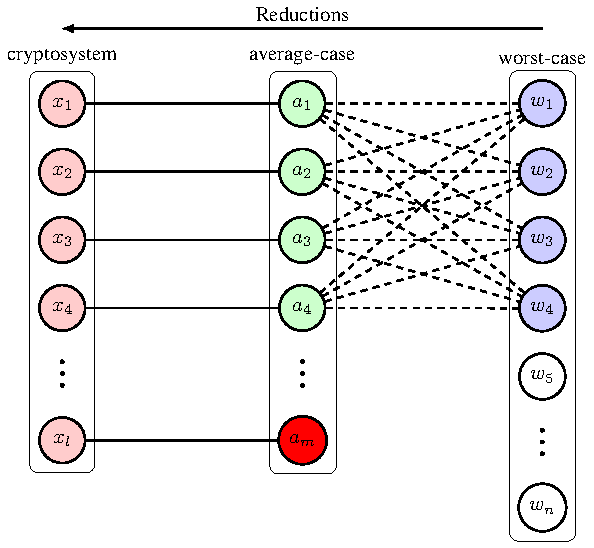
\includegraphics[page=1]{images/Lattice_crypto_tikz_folder.pdf}
    \caption{A demonstration of a cryptosystem's computational security that is based on an average-case problem. Each cryptographic instance $x_i$ corresponds to a random average-case instance $a_j$. All random instances in the average-case problem can be mapped with the hard instances in the worst-case problem. There may be a fraction of average-case instances (colored in red) that can be solved easily, so their solutions entail solutions of the worst-case problem. But the fraction of such instances is negligible. The hard and easy instances in the worst-case problem are colored blue and white, respectively. The dashed lines indicate the worst-case-to-average-case reduction is random.}
    \label{fig:average2worstDuplicate}
\end{figure}
%https://www.youtube.com/watch?v=qZIjVX61NFc&t=433s&ab_channel=SimonsInstitute, at 39mins
\fi

A couple of remarks about the reduction. First, the approximation (or gap) factors in the lattice problems are relatively large, typically larger than $n^8$ as analysed by \citet{cai1997improved} and suggested in the Introduction section in \citep{micciancio07worst}. This could raise minor concerns about the hardness of the lattice problems, because the larger the gap factors the easier the problems are. In a following section, we will introduce the discrete Gaussian strategy to reduce these factors down to $\tO(n)$ for the SIS problem.
The proof strategy will follow Ajtai's technique of constructing, from a set of linearly independent vectors of a lattice, a random set of lattice vectors that are well spread out and as short as possible.
Second, the public key size required by an SIS-based cryptosystem is $\tO(n^4)$ that is quite inefficient for practical purposes. This will be dramatically improved by developing different average-case problems as we will see in the learning with error and ring learning with error problems. 
%Read Section 1.1 in \citep{micciancio07worst} for a more detailed interpretation of earlier techniques on worst-case-to-average-case reductions.

%\kl{what's the gap factor? mention it here, because we will introduce an improvement using discrete Gaussian.}


\subsection{An application of SIS: Collision resistant hash functions}

SIS has been used as the foundation of one-way functions and hash functions, see e.g. \citep{lyubashevsky2010ideal}.

%
% \textcolor{red}{This stuff about one-way functions might be a bit of a distraction. What we really want to say is that the SIS problem lets us build a collision resistant hash function.  I'm not really happy with describing the SIS function as a one-way function. Really, all it guarantees is that it's hard to find a preimage for 0.  Collision resistance is usually a stronger property than preimage resistance, but not always.  I think we'd need to be more careful than we really want to be to make everything here bulletproof. I've commented out some things about one-way function as a suggestion for a cleaner, and shorter, exposition.}

% The SIS problem can be viewed as a one-way function because given such a solution it is easy to compute the zero vector output, but going backwards to infer such a integer vector from the solution is difficult. It was later proved to be a collision resistant hash function, which is an even stronger cryptographic primitive. 

% Let $f: \{0,1\}^* \rightarrow \{0,1\}^*$ be a function. For any algorithm $\mathcal{A}$ and a security parameter $n$, define the \textbf{inverting experiment} \textbf{Invert}$_{\mathcal{A},f}(n)$ as: 
% \reversemarginpar
% \marginnote{\textit{\textbf{Invert}$_{\mathcal{A},f}(n)$}}
% \begin{enumerate}
%     \item Choose uniform $x \in \{0,1\}^*$ and compute $y=f(x)$.
%     \item Run the algorithm $\mathcal{A}(y) \rightarrow x'$.
%     \item \textbf{Invert}$_{\mathcal{A},f}(n)=1$ if $f(x')=y$ and 0 otherwise. 
% \end{enumerate}

% This gives rise to the definition of one-way functions.

% \begin{definition}
% A function $f: \{0,1\}^* \rightarrow \{0,1\}^*$ is \textbf{one-way} 
% \reversemarginpar
% \marginnote{\textit{One-way function}}
% if it satisfies the following two conditions:
% \begin{itemize}
%     \item $f(x)$ is computable in polynomial time. 
%     \item For any probabilistic polynomial time adversary $\mathcal{A}$, $Pr[\textbf{Invert}_{\mathcal{A},f}(n)=1] \le \text{negl}(n)$.
% \end{itemize}
% \end{definition}

A hash function maps inputs of arbitrary length and compresses them into short fixed-length outputs known as \emph{digests}.

\begin{definition}
A \textbf{(keyed) hash function} \index{hash function}
\reversemarginpar
\marginnote{\textit{Hash function}}
with output length $l$ is a pair of probabilistic polynomial-time algorithms $(\text{Gen},H)$ satisfying the following: 
\begin{itemize}
    \item The algorithm $\text{Gen}(1^n) \rightarrow s$ generates a key $s$ from the security parameter $1^n$.
    \item For a string $x\in \{0,1\}^*$ of arbitrary length, the algorithm $H$ outputs a string $H^s(x) \in \{0,1\}^{l(n)}$.
\end{itemize}
\end{definition}

The general interest in hash functions is the case when the outputs are shorter than the inputs for both computational and storage efficiency. In such a case,  a hash function's domain is larger than its range, which implies the possibility of having two distinct inputs being mapped to the same output. We often say the two distinct inputs \textit{collide} and the scenario is called a \textit{collision}. 

For a hash function $\Pi=(\text{Gen},H)$, an adversary $\mathcal{A}$ and the security parameter $n$, we can define the \textbf{collision-finding experiment} \textbf{Hash-coll}$_{\mathcal{A},\Pi}(n)$ as:
\reversemarginpar
\marginnote{\textit{\textbf{Hash-coll}$_{\mathcal{A},\Pi}(n)$}}
\begin{enumerate}
    \item Run the algorithm $\text{Gen}(1^n) \rightarrow s$. 
    \item The adversary $\mathcal{A}$ is given the key $s$.
    \item The adversary produces two strings $x$, and $x'$.
    \item \textbf{Hash-coll}$_{\mathcal{A},\Pi}(n)=1$ if $x \neq x'$ and $H^s(x)=H^s(x')$ and 0 otherwise.  
\end{enumerate}

A cryptographic hash function requires the chance of finding a collision is negligible, which is defined more formally as follows. 
\begin{definition}
A hash function $\Pi=(\text{Gen},H)$ is \textbf{collision resistant} \index{hash function! collision resistant}
\reversemarginpar
\marginnote{\textit{Collision resistant}}
if for any probabilistic polynomial time adversary $\mathcal{A}$, it satisfies 
\begin{equation*}
    Pr[\text{Hash-coll}_{\mathcal{A},\Pi}(n)=1] \le \text{negl}(n).
\end{equation*}
\end{definition}

From Ajtai's SIS problem and the worst-case-to-average-case reduction, one can easily build a collision resistant hash function where the key is the matrix $A \in \Z_q^{n \times m}$ and the hash function is given by 
\begin{align*}
    &f_A: \{0, \dots, d-1\}^m \rightarrow \Z_q^n \\
    &f_A(\mathbf{x})=A\mathbf{x} \bmod q.
\end{align*}
If there is a collision $f_A(\vc{x})=f_A(\vc{x'})$ between distinct inputs $\vc{x}$ and $\vc{x'}$, then $A(\vc{x}-\vc{x}^{\prime}) = 0$ and $\vc{x} - \vc{x}^{\prime} \in L^{\perp}_q(A)$. Furthermore, because each element of $\vc{x} - \vc{x}^{\prime}$ is in the set $\{-1,0,1\}$, we see that $\vc{x} - \vc{x}^{\prime}$ is a short vector. Hence, an efficient algorithm that produces collisions for this hash function could be used to solve SIS in the lattice $L^{\perp}_q(A)$. 

% We already said all of this in the last paragraph of the previous subsection.
% This hash function is easy to be implemented, but its efficiency is a drawback due to the quadratic size of the key matrix $A$. Furthermore, the larger a gap is, the easier a gap problem is. This leads to subsequent works of relying the security of average-case problems on worst-case lattice problems with smaller gaps. Improvements based on Ajtai's work and other variations were done using different constructions and advanced algebraic structures such as \textit{ideal lattices}. We will discuss these in details in later sections. 

\iffalse 
Usually, we analyse the complexity of an algorithm for a computational task on all possible inputs. This corresponds to the \textit{worst-case complexity}. For example, the definition of NP-completeness for decision problems. When solving a computational problem in practice, however, the worst cases may have very low probabilities of being encountered. This can either be good or bad, depending on what the computational problem will be used for. For example, the 3-colouring problem (that is NP-complete) can be solved in linear time for most random graphs. But if the security of a cryptosystem is based on the worst-case hardness of the 3-colouring problem, then most of the system's encryption can be attacked easily. 

Similar to problems that are (worst-case) NP-hard, there are problems that are average-case hard too, namely \textbf{distNP-hard}. 

Average-case hardness is a stronger assumption than worst-case hardness, as if a problem is average-case hard then it must be worst-case hard, but not vice versa. 
Below are some remarks on average-case complexity. For more detail, see Chapter 18 of \citep{arora2009computational}. 
\begin{itemize}
    \item The average-case problem consists of a decision problem and a distribution from which inputs can be sampled in polynomial time. 
    
    \item Average-case complexity is defined with respect to a particular distribution on the inputs. A problem may be difficult with one distribution but easy with another distribution.  
    
    \item Similar to P and NP for the worst-case complexity, average-case complexity has computational classes \textbf{distP} and \textbf{distNP}. 
\end{itemize}

Worst-case hard problems are relatively easier to be proved as it is sufficient to build polynomial time Turing reductions from known NP-complete problems. In contrast, average-case hard problems are more difficult to be proved in general. From the perspective of building secure cryptosystems, on the one had, the fact that random cases of average-case hard problems are difficult to be solved efficiently is an advantage. On the other hand, worst-case hardness is weaker than average-case hardness, so worst-case hardness is a more preferable assumption for building secure cryptosystems. Therefore, it would be an ideal situation if cryptosystems security can be based on worst-case hard problems and there are systematic ways of randomly generating those worst cases. This is exactly what some lattice-problems can provide due to the breakthrough of \cite{ajtai1996generating}'s work.

\citet{ajtai1996generating} proved that some lattice problems are ...
\fi 

\iffalse
\textcolor{blue}{KS: For a chronological listing of results starting from Ajtai, have a look at Section 4 of \cite{micciancio11lattice}. For an actual proof that's easy to describe, we may want to describe the one in \cite{micciancio07worst}, but without the advanced technical bells and whistles.
}
\fi
\iffalse
\textcolor{blue}{KS: Note that, in the design of a crypto-system, there is a distinction in the basic design steps depending on whether one is assuming an average-case hard problem $\mathit{ACH}$ or a worst-case hard problem $\mathit{WCH}$.}

\textcolor{blue}{In constructing a crypto-system using an $\mathit{ACH}$, it's sufficient to show that the generation of a key pair (at random) and the solution of the private key corresponds to a problem instance $I \in \mathit{ACH}$, and we rely on average hardness to say $I$ is hard to solve with good probability.}

\textcolor{blue}{In constructing a crypto-system using an $\mathit{WCH}$, we need to do a bit more work, in that it's not sufficient to generate a key pair (at random) and show the solution of the private key is a problem instance $I \in \mathit{WCH}$, we need to actually show that $I$ is close to the worst cases in $\mathit{WCH}$.
}

\textcolor{blue}{It's true that building a crypto-system using a worst-case hard problem is more attractive because it relies on a weaker assumption, but with that weaker assumption comes more work. 
In particular, for many worst-case hard problem classes, we don't actually know how to generate the worst cases (or hard cases close to the worst cases) so they can't be used in the design of a crypto-system. The nice thing about lattice problems is that they are both worst-case hard \emph{and} we know how to generate those hard problem instances. 
}

\textcolor{blue}{
Note also that the Discrete Logarithm and Integer Factorisation problems, which underlie several well-known crypto-systems, are only known to be in NP, they are not known to be in NP Complete or NP Hard. The way we understand their complexity is by generating random instances of Discrete Log and Integer Factorisation problems and then seeing how long the current best known (non-polynomial) algorithms for those two problems will take to solve the problem. Using that heuristic complexity measure, we can show that (1) there are special instances of those problems that can be solved in polynomial time but, in general, both problems can be solved only in sub-exponential time and (2) on average, most of the Discrete Logarithm and Integer Factorisation problem instances are as hard as each other. So we *believe* these two problems to be average-case hard problem classes, but we can't prove that. Interestingly, we know there are quantum algorithms that can solve these two problems efficiently.}
\fi 

\iffalse
\textcolor{blue}{Lattice problems like SVP, GVP, however, have been proven to be NP Hard under the "randomised reduction hypothesis", in which the class of polynomial-time algorithms is enlarged to include those are not deterministic but will, with high probability, terminate in polynomial time with a correct result. This is basically Ajtai's result. The NP-hard-ness of lattice problems is also why crypto-systems built on top of them are safe from quantum computing, whereas crypto-systems built on top of Discrete Log or Integer Factorisation are not.
}
\fi

%%%%%%%%%%%%%%%%%%%%%%%%%%%%%%%%%%%%%%%%%%%%%%%%%%%%%%%%%%%%%%%%%%%%%%%%%%%%%%%%%%%%%%%%%%%%%%%%%%%

%\newpage
%\bibliography{references}
%\bibliographystyle{abbrvnat}

\end{document}